\section{Software architecture}

\begin{figure}
  \centering
  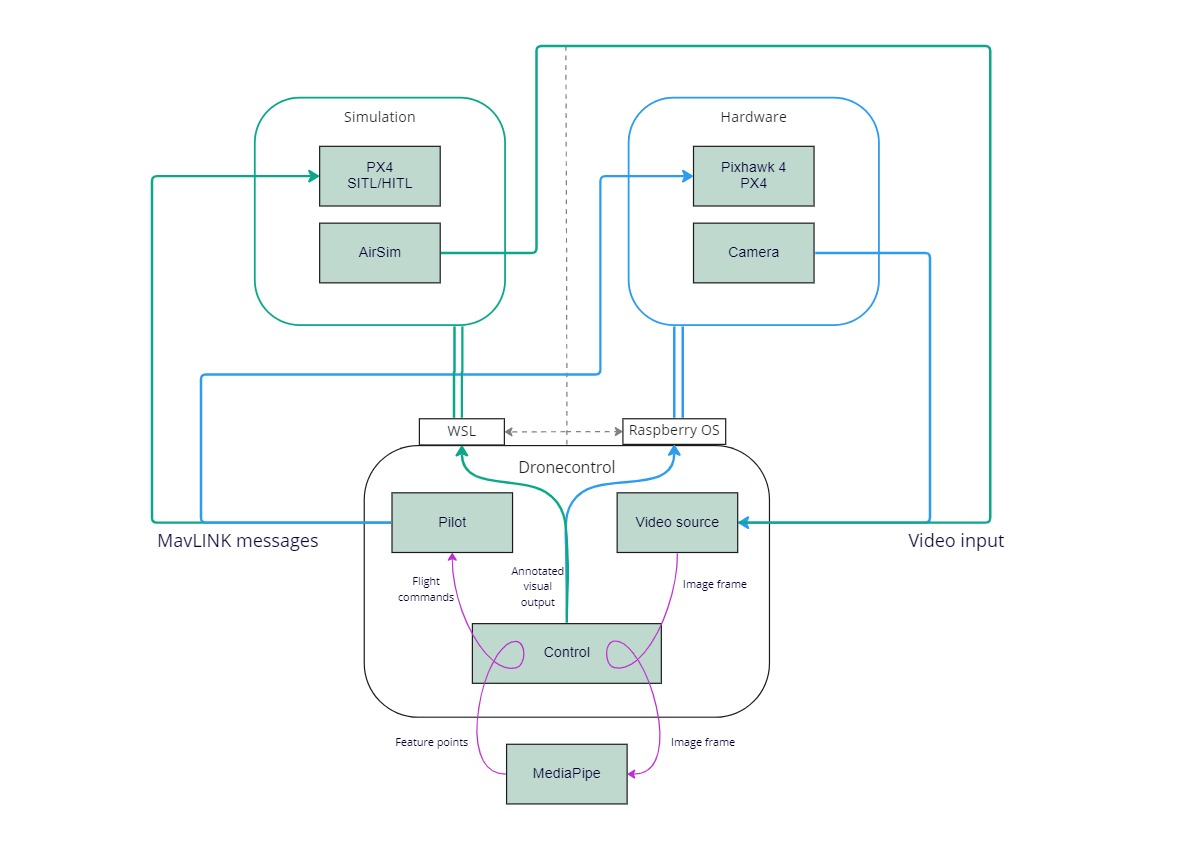
\includegraphics[width=\textwidth, keepaspectratio]{img/software-arch.jpg}
  \caption{Structure of the program}\label{fig:architecture}
\end{figure}

\todo[inline]{Write: Describe the actual new diagram, blue vs green arrows, data flow, ...}

Figure \ref{fig:architecture} shows the main modules the designed the software is composed of and how it interacts with the external libraries.
The application consists of three basic parts: 
the pilot module, in charge of sending instructions to the flight controller and receiving back information on position and state through the \texttt{mavsdk} library, 
a video source module that handles the retrieval of images from different sources and the necessary processing for image analysis, 
and a control module that directs the interaction between the other two to transform the pixel information first into position points through the \texttt{mediapipe} library and then into instructions for the pilot.
The upper part of the diagram in figure \ref{fig:architecture} shows how the program modules receive input and send instructions to the hardware systems whether these are simulated or not.
Other smaller utilities have also been developed to help test how the systems interact with each other and calibrate different parts of the control behaviour.
Appendix \ref{app:cli} contains the user manual with all the application's options.

\subsection{Pilot module}
The purpose of the pilot module is to provide access to the rest of the application to send and receive messages from the PX4 controller through the MavSDK library.
This library provides a simple asynchronous API for managing one or more vehicles, providing programmatic access to vehicle information and telemetry, and control over missions, movement and other operations.
MavSDK utilizes the python standard library \emph{asyncio} to be able to run coroutines in parallel while waiting for the messages provided through the \emph{MAVLink} communication.
Therefore all calls to the library have to be written as async functions that await the result of one or more polls to the flight stack.

\texttt{asyncio} provides support for writing concurrent code using the \texttt{async/await} syntax.
It is used as a foundation for multiple Python asynchronous frameworks that provide high-performance network and web-servers, database connection libraries, distributed task queues, etc; 
and provides a set of high-level APIs to run Python coroutines concurrently and have full control over their execution.
The pilot module integrates \texttt{mavsdk} and \texttt{asyncio} and provides a queue for the control module to send actions to be executed in the vehicle one after another.

Listing~\ref{lst:pilot.connect} shows how to establish a connection to a PX4 vehicle through its physical (serial) or virtual (UDP) address and poll for internal information from the flight controller to decide when the system is ready to receive instructions.
The mavsdk library exposes telemetry and other state information through asynchronous generators, which are defined in python as a convenient way to make asynchronous data producers and accessed with the \mintinline{python}{async for} syntax.


\begin{listing}[h!]
    \caption{Example of how the communication to the flight stack is established through asyncio and the mavsdk library}{}
    \label{lst:pilot.connect}
    \begin{minted}[breaklines, fontsize=\footnotesize, baselinestretch=1]{python}
async def connect(self):
    """Connect to mavsdk server.
       Raises a TimeoutError if it is not possible to establish connection.
    """
    
    if self.serial:
        address = f"serial://{self.serial}"
    else:
        address = f"udp://{self.ip if self.ip else ''}:{self.port}"
    self.log.info("Waiting for drone to connect on address " + address)
    await asyncio.wait_for(self.mav.connect(system_address=address), timeout=self.TIMEOUT)

    async for state in self.mav.core.connection_state():
        if state.is_connected:
            break

    # Wait for drone to have a global position estimate
    async for health in self.mav.telemetry.health():
        if health.is_global_position_ok:
            break
        
    self.log.info("System ready")
    self.is_ready = True
    \end{minted}
\end{listing}

Many of basic operations that can be executed in the flight controller are implemented in the pilot module with error handling and safety checks, like takeoff, landing, return home or manipulating the vehicle flying velocity directly by providing speeds in body coordinates.
These actions can be executed directly or added to a queue that runs in on a loop executing them in the order they are added, waiting until the previous action has finished and the vehicle is in the desired state before starting the next.
The loop that runs this queue can be seen in Listing~\ref{lst:pilot.queue}.
There is a maximum time of 10 seconds that each action can use to run
The loop stops when the asynchronous task it runs on is cancelled with \mintinline{python}{task.cancel()}, which raises a \mintinline{python}{CancelledError} exception in the parallel execution.

\begin{listing}[h!]
    \caption{Loop where the action queue runs on the pilot module. Each action is awaited until it finishes or the timeout time runs out.}{}
    \label{lst:pilot.queue}
    \begin{minted}[breaklines, fontsize=\footnotesize, baselinestretch=1]{python}
async def run_queue(self):
    """
    Run the queue loop.
    
    Queued actions will be awaited one at a time
    until they are finished.
    The loop will sleep if the queue is empty.
    """
    try:
        while True:
            if len(self.actions) > 0:
                action = self.actions.pop(0)
                self.log.info("Execute action: %s", action.func.__name__)
                try:
                    await asyncio.wait_for(action.func(self, **action.args), timeout=10)
                except asyncio.exceptions.TimeoutError:
                    self.log.warning(f"Time out waiting for {action.func.__name__}")
            else:
                await asyncio.sleep(self.WAIT_TIME)
    except asyncio.exceptions.CancelledError:
        self.log.warning("System stop")
    \end{minted}
\end{listing}

\subsection{Video source module}

The objective of the video source module is to provide a collection of classes to retrieve images from different sources,
in a way that they can be exchanged for one another without affecting the rest of the application to facilitate testing and be adaptable running in different environments.
There are three classes of video sources implemented: file, simulator and camera, which inherit from the same \mintinline{python}{VideoSource} base class as shown in Figure~\ref{fig:video-source-inheritance}.

\begin{figure}
  \centering
  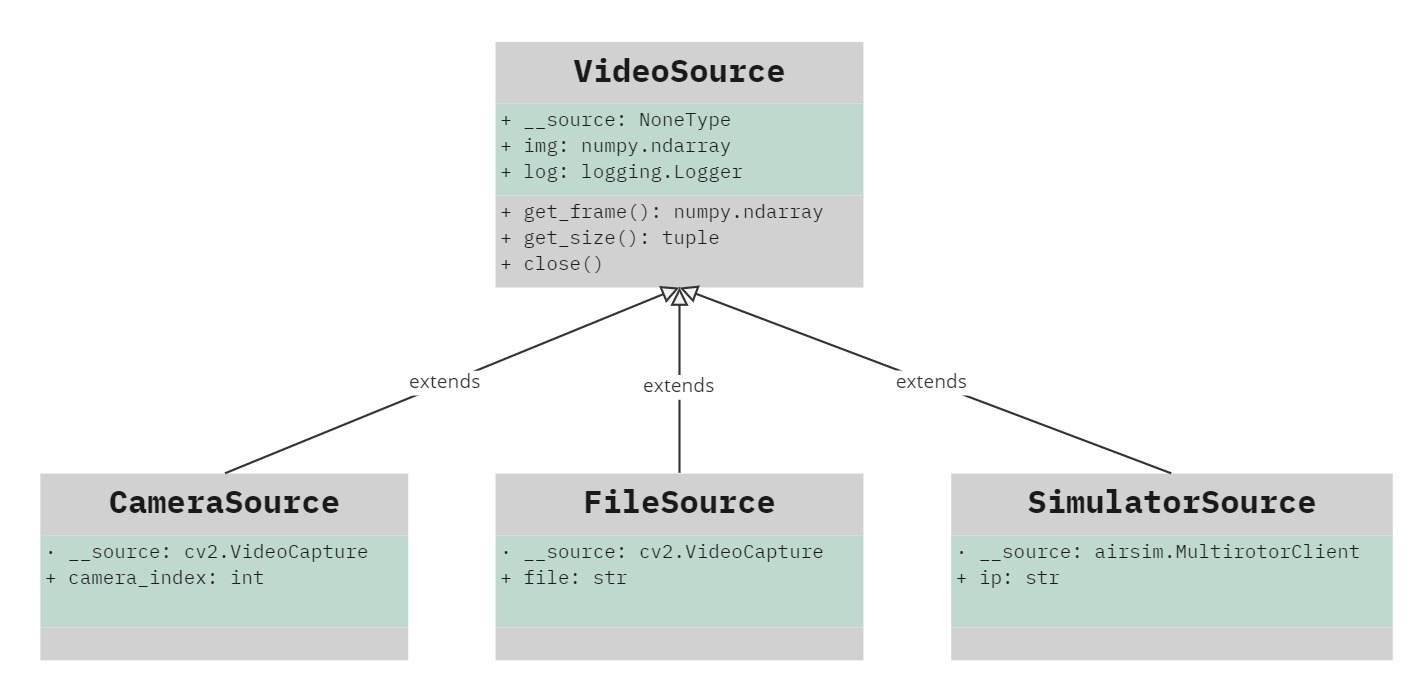
\includegraphics[width=8cm, keepaspectratio]{img/uml-video-source.jpg}
  \caption{Diagram of inheritance on the video source classes available to retrieve image data.}
  \label{fig:video-source-inheritance}
\end{figure}

The \mintinline{python}{FileSource} class is able to open a video file stored in the companion computer and provides images taken frame by frame from it until the video ends.
This allows the program to replay the image detection algorithms on videos previously captured by the camera tool exposed in section~\ref{subsec:test-tools}.
The \mintinline{python}{CameraSource} class can access a physical camera attached to the computer running the application via USB and provide the frames captured in real time.
Both the file and camera sources employ OpenCV's video capture utilities to take care of the file handling and the camera driver management capabilities respectively.

The simulator source uses AirSim's Python library to communicate with the simulator and retrieve images from a simulated camera attached to the 3D model of the vehicle in Unreal Engine.
It connects automatically through localhost, but it can also be provided with an IP to establish connection to the simulator running on a different computer on the local network, for example when the program runs inside WSL and the simulator runs on its host computer.

\subsection{Vision control module}
The control module contains the main logic of the application and is in charge of converting the raw images obtained from the video source into commands for the pilot module.
Two different types of control have been implemented.
The first one is a proof-of-concept control solution, described in section \ref{sec:hands}, that runs in offboard mode (see section \ref{subsec:offboard}) and translates some predefined hand gestures into simple commands for the aerial vehicle, of which the main purpose is to be able to test the interaction between all the components of the system in a more easily controlled environment, since it uses the simpler configuration of situating the computer with the controller outside of the vehicle.
The second control system consists of a follow solution more applicable to real-life scenarios where the control and the camera is onboard the vehicle and the presence of a person is detected in the images obtained from the perspective of the drone in order to be able to give the flight controller velocity commands to follow said person and maintain it centered in its view.

The process followed in both solutions consists roughly of the same two parts.
First the image is sent to the computer vision and machine learning third-party library that extracts the required features from the image in the form of 2D coordinates.
Afterwards a series of calculations depending on the particular solution are applied to these coordinates to decide which commands are sent to the pilot module.
The third-party library used for computer vision in the program is the mediapipe library described in Section~\ref{subsec:mediapipe}, which offers cross-platform, customizable ML solutions for live and streaming media, specifically its hand and pose detection solutions.

To engage the module in direct control of the vehicle's velocity it is necessary to use a special flight mode defined by PX4 for this purpose, called Offboard Mode \footnote{\url{https://docs.px4.io/main/en/flight_modes/offboard.html\#offboard-mode}} (not to be confused with the offboard configuration described in section~\ref{subsec:offboard}).
Offboard mode is primarily used for controlling vehicle movement and attitude, and supports only a very limited set of MAVLink messages. This mode requires position or pose/attitude information to be available to the flight controller, e.g. GPS.
In it, the vehicle obeys a position, velocity or attitude setpoint provided over MAVLink by a MAVLink API (i.e. MAVSDK) running on a companion computer and usually connected via serial cable or wifi.
A stream of setpoint commands must be received by the vehicle at a rate higher than 2Hz prior to engaging the mode and in order to remain in it.
If the message rate falls below 2Hz or the connection is lost the vehicle will stop and, after a timeout, the vehicle will attempt to land or perform some other failsafe action according to the parameters configured.
In order to hold position while in this mode, the vehicle must receive a stream of setpoints for the current position.

Sections~\ref{sec:hands} and \ref{sec:follow} offer a more complete explanation of the control module used by the two different solutions developed.

\subsubsection{Camera-testing tool}
\label{subsec:test-tools}

Several additional utilities have been added to the dronecontrol program to facilitate the development and testing process of the two main control solutions.
The first tool is accessed through the command \mintinline{bash}{dronecontrol tools test-camera} and can be used for testing the connection between the computer and the camera, as well as the performance of the MediaPipe hand and pose machine learning solution on real time images.
It is as well possible to take images and record video from the live camera feed for later analysis and it allows connecting to a physical or simulated flight controller to send basic commands through keyboard input like takeoff and landing.

\todo[inline]{Write: Add control functionality, describe connection options, link to cli in appendix}
\todo[inline]{Polish: Link some code from test-camera tool}





\section{Proof of concept: hand-gesture solution}
\label{sec:hands}
The main purpose of this solution is to test that the flow of the application works as expected, both in simulation and in real flight, and that all the systems are capable of establishing the required connections with each other.
For that reason it is designed to be able to be run in real flight with the minimal setup of a built drone with its default components and any computer with a camera.

\begin{figure}
  \centering
  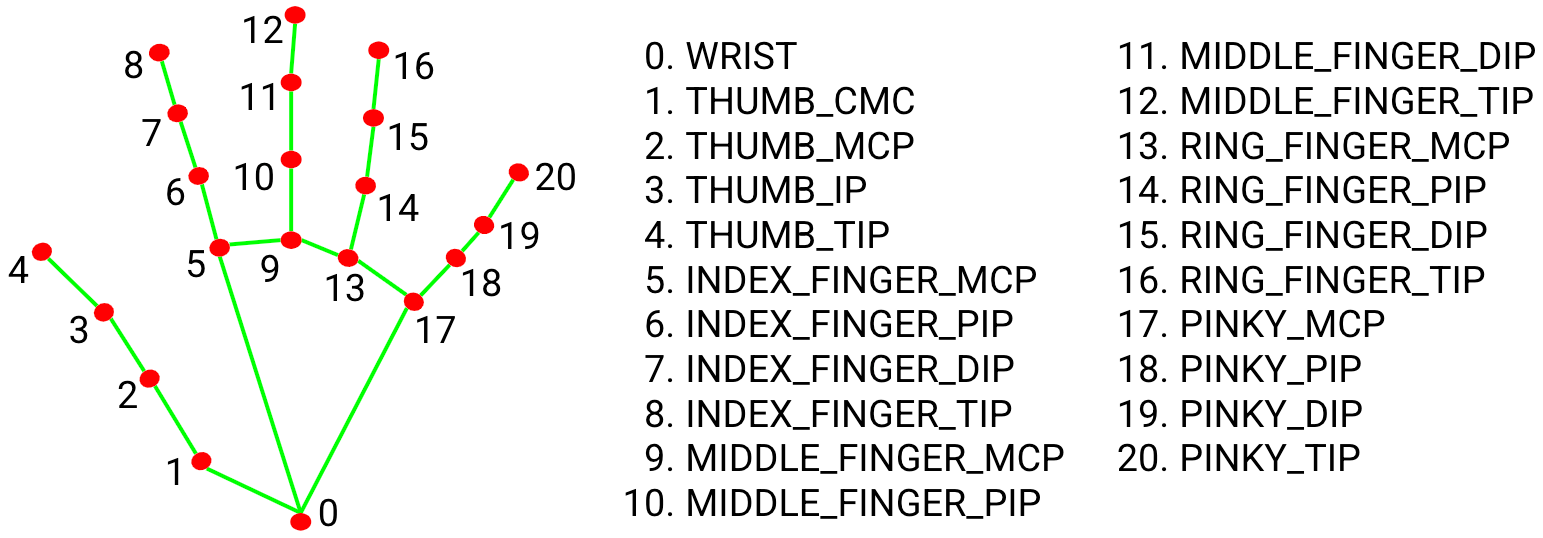
\includegraphics[width=\textwidth, keepaspectratio]{img/hand_landmarks.png}
  \caption{Landmarks extracted from detected hands by the MediaPipe hand solution.}
  \source{Adapted from \citetitle{mp-hands} \cite{mp-hands}.}
  \label{fig:hand-landmarks}
\end{figure}

This control module runs on a loop that continuously polls for a new frame from the chosen video source and feeds it to the hand detection functionality from MediaPipe \cite{mp-hands-paper}.
If a hand is detected in the images, 2D coordinates are extracted according to the map shown in figure~\ref{fig:hand-landmarks}.
These landmarks are then converted into different discrete gestures like open palm, closed fist or an specific finger pointing different directions.
When a new gesture is detected, the command assigned to it is queued to the pilot module and executed as soon as the previous commands end their execution.

The conversion between landmarks and gestures is performed by drawing vectors from the base of each of the fingers to their tips as well as from the base of the hand (wrist feature) to the base of the fingers and using the dot product vector operation to calculate the relative angles between each finger and the base of the hand, as shown in figure~\ref{fig:vector-calcs}.
By comparing the calculated angles to a threshold, it is possible to detect whether each individual finger is extended or folded, as well as the general direction it is pointing towards.
The open hand gesture, for example, can then be defined as all five fingers extended, that is, all five vectors defined by the fingers sharing the same approximate angle with the vector from the base of the hand to that finger.

\begin{figure}
  \centering
  
\includegraphics[width=8cm, keepaspectratio]{img/placeholder.png}
  \caption{Vector calculations}
  \label{fig:vector-calcs}
\end{figure}
\todo[inline]{Draw: hand vectors}

The full list of gestures detected by the program by calculating these angles is as follows:
\begin{itemize}
    \item No hand: happens when no landmarks are able to be extracted from the image. As a safety feature, in this case the vehicle stops whichever previous commands it had in its queue and goes into hold flight mode, where it just hovers in the air maintaining its position.
    \item Open hand: it is detected when all five fingers are extended, as if gesturing stop, and makes the drone land at its current position.
    \item Fist: it is detected when all five fingers are folded and makes the drone arm and takeoff. If the drone is already in the air nothing happens.
    \item Index finger pointing up: it is detected when only the index finger is extended and it is pointing roughly towards the top of the image ($\pm 30$ degrees) and makes the drone go into offboard mode, where it is possible to receive direct velocity commands.
    \item Index finger pointing to the right: same as above but pointing to the right of the image and makes the drone roll towards its right side at a speed of 1 m/s.
    \item Index finger pointing to the left: same as above but the drone rolls towards its left side.
    \item Thumb pointing to the right: it is detected when index finger is extended up (to maintain the drone in offboard control) and the thumb is extended pointing towards the right of the screen. This gesture makes the drone pitch forward at a steady speed of 1 m/s.
    \item Thumb pointing to the left: same as the previous gesture, but the drone pitches backward when the thumb point to the left of the screen.
\end{itemize}

\todo[inline]{Write: add loop code and link to first paragraph}
\todo[inline]{Draw: Include diagram of angles for each pointy gesture ?????}
\todo[inline]{Images: simulators program output image with drawn lines for gestures}
\todo[inline]{Video: hand control in simulator}





\section{Final solution: human following}
\label{sec:follow}

The intention behind the development of a UAV control solution that implements tracking and following of humans is to show how the PX4 open-source development platform and its related projects, MAVLINK and MAVSDK, can be used to design complex real-life applications without the need for expensive state-of-the-art proprietary hardware.
The only requirements of the follow application are a PX4-enabled flight controller installed in an aerial vehicle, a companion computer of appropriate dimensions to be able to be mounted on board the vehicle and any camera that can be connected to the companion computer via USB.
During the program execution, the drone can be controlled via an RC controller, an external ground station application or keyboard input directly to the companion computer through, for example, a secure shell using the SSH protocol.

For safety, the follow mechanism only engages when the flight mode on the vehicle is changed to offboard mode e.g. by activating a configured switch in the RC controller, and stops automatically if the connection to the computer is lost or any of the available failsafes are triggered, like low battery, loss of RC or GPS signal or vehicle attitude exceeding a predefined pitch and roll value for longer than a specified time.
In this mode the vehicle will attempt to find a single person in its field of view and follow their movements by changing its yaw and forward velocity to match horizontal movements and distance changes, respectively.

\begin{figure}
  \centering
  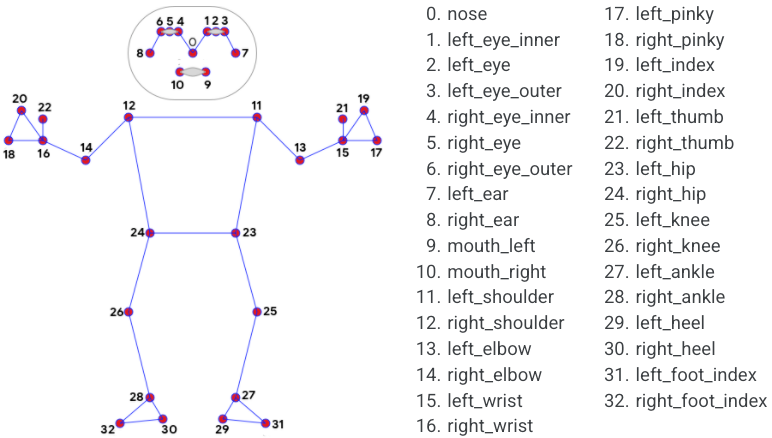
\includegraphics[width=\textwidth, keepaspectratio]{img/pose-landmarks.png}
  \caption{Landmarks extracted from detected human figures by the MediaPipe Pose solution}
  \source{Adapted from \citetitle{mp-pose} \cite{mp-pose}}
  \label{fig:pose-landmarks}
\end{figure}

During the program execution and while the offboard mode and the follow mechanism is engaged, the system continuously retrieves images from the offboard camera that are fed into the MediaPipe Pose \cite{mp-pose-paper} computer vision library to extract pose landmarks from it in the form of 2D coordinates.
Figure~\ref{fig:pose-landmarks} shows the available extracted features and their correspondence to the human body.
These coordinates are used to draw a bounding rectangle around the detected person, as well as for validating that the received landmarks match the general pose of a person standing up.
To prevent unwanted movements, the vehicle will always stop and hover every time it becomes impossible to detect a person in the image received or its features do not match the expected geometry.
\todo[inline]{Images: valid and invalid person detection from simulator camera output}
After a valid bounding box has been defined around the target person, its position in respect to the field of view of the camera is sent to a control mechanism composed of two independent PID controllers. The theory behind these controllers is explained in section~\ref{subsec:pid-tools}).

The first of the PID controllers is in charge of controlling the yaw velocity of the vehicle to respond to horizontal movements in the x direction of the image. 
\todo[inline]{Draw: coordinate system figure}
It takes as input the x coordinate of the center point of the bounding box and its target is the middle point of the screen.
This controller therefore will output velocity commands aimed to maintain the bounding box centered horizontally in its field of view.

The second PID controller controls the forward velocity of the vehicle to respond to distance changes of the person getting closer or further away from the drone.
It takes as input the height of the calculated bounding box as a percentage of the total height of the field of view and works to keep it within a value that matches the desired distance to maintain between the person and the vehicle by moving forwards when the height is too low and backwards when it is to high.
The exact percentage of the image height that is covered by a person at a given distance depends on the camera used and needs to be obtained empirically for each separate video source.

\todo[inline]{Add some controller and follow code to show and explain}
\todo[inline]{Images: simulator and output, link video of run}



\subsubsection{PID tools}

Two additional utilities have been developed for tuning and measuring the performance of the PID controllers.
\todo[inline]{Write: PID tools, how they work and code}
\todo[inline]{PID library, Formula and coefficients}

%%%%%%%%%%%%%%%%%%%%%%%%%%%%%%%%%%%%%%%%%
\begin{equation}
    u(t)= K_p e(t) + K_i \int{e(t)dt} + K_d \frac{de(t)}{dt}
%    \caption{Formula for the output from a PID controller}
    \label{eq:pid}
\end{equation}
%% Where: $u(t)=$ PID control variable
        % $K_p=$ proportional gain
        % $K_i=$ integral gain
        % $K_d=$ derivative gain
        % $e(t)=$ error value
        % $de=$ change in error value
        % $dt=$ change in time
%%%%%%%%%%%%%%%%%%%%%%%%%%%%%%%%%%%%%%%%%

The process of tuning the PID controllers is described in section~\ref{sec:test-1-pid}


\subsection{Safety mode}
\label{subsec:safety}

\todo[inline]{Write: safety mechanisms, speed limits on pids, loss of signal, loss of vision, ...}
\todo{}
\todo{}

